\documentclass[11pt,letterpaper]{article}
\usepackage[utf8]{inputenc}
\usepackage[T1]{fontenc}
\usepackage[spanish,es-tabla,es-nodecimaldot]{babel}
\usepackage{mathptmx}
\usepackage[letterpaper,margin=2.5cm]{geometry}
\usepackage{amsmath,amssymb,amsthm}
\usepackage{booktabs,array,longtable}
\usepackage{graphicx}
\usepackage{enumitem}
\usepackage{xcolor}
\usepackage{tcolorbox}
\tcbuselibrary{breakable}
\usepackage[stretch=10,shrink=10]{microtype}
\usepackage{url}
\usepackage{hyperref}
\definecolor{upblue}{RGB}{17,68,135}
\hypersetup{colorlinks=true,linkcolor=upblue,urlcolor=upblue,citecolor=upblue,
  pdftitle={El SIC y la liquidez del mercado accionario mexicano: notas de clase}}
\setlength{\parindent}{0pt}
\setlength{\parskip}{0.55em}
\emergencystretch=3em
\setlist{itemsep=2pt,topsep=3pt}
\makeatletter
\g@addto@macro{\UrlBreaks}{\do\/\do\-\do\.\do\_\do0\do1\do2\do3\do4\do5\do6\do7\do8\do9}
\newcommand{\tablainput}[1]{\@@input #1.tex }
\makeatother

\theoremstyle{definition}
\newtheorem{definicion}{Definición}[section]
\newtheorem{ejemplo}[definicion]{Ejemplo}
\theoremstyle{plain}
\newtheorem{proposicion}[definicion]{Proposición}
\newtcolorbox{leccion}{colback=upblue!5,colframe=upblue!70,boxrule=0.5pt,arc=1pt,breakable,
  fontupper=\small,before upper={\textbf{Lección.}\ }}
\newtcolorbox{cambio}{colback=orange!6,colframe=orange!70!black,boxrule=0.5pt,arc=1pt,breakable,
  fontupper=\small,before upper={\textbf{Qué cambia respecto de la tesis.}\ }}
\newenvironment{ejercicios}{\par\medskip\textbf{Ejercicios}\begin{enumerate}[label=\arabic*.,leftmargin=*]\small}{\end{enumerate}}

\newcommand{\PSIC}{\mathit{PSIC}}
\newcommand{\ILLIQ}{\mathit{ILLIQ}}
\newcommand{\ZRET}{\mathit{ZRET}}
\newcommand{\TURN}{\mathit{TURN}}
\newcommand{\SPREAD}{\mathit{SPREAD}}
\DeclareMathOperator{\logit}{logit}
\newcommand{\web}[1]{\textsuperscript{[#1]}}

% Generado por scripts/notas_analisis.py. No editar a mano.
\newcommand{\RtHAC}{13.61}
\newcommand{\RpendHAC}{2.17}
\newcommand{\RadfLogit}{0.207}
\newcommand{\RkpssLogit}{0.010}
\newcommand{\RderivaAnual}{0.151}
\newcommand{\RtDeriva}{1.03}
\newcommand{\RpDeriva}{0.303}
\newcommand{\RlagNW}{4}
\newcommand{\RderivaA}{0.214}
\newcommand{\RpDerivaA}{0.473}
\newcommand{\RderivaB}{0.318}
\newcommand{\RpDerivaB}{0.078}
\newcommand{\RderivaC}{-0.036}
\newcommand{\RpDerivaC}{0.824}
\newcommand{\RrwRechazo}{82}
\newcommand{\RrwMediana}{6.0}
\newcommand{\RratioDosMilTrece}{353}
\newcommand{\RratioDosMilVeinticuatro}{175}
\newcommand{\RamibDosMilCuatro}{1.13}
\newcommand{\RamibCorregido}{2.24}
\newcommand{\RbbgDosMilCuatro}{3.13}
\newcommand{\RillNomA}{-3.78}
\newcommand{\RillRealA}{-3.38}
\newcommand{\RillNomB}{3.01}
\newcommand{\RillRealB}{3.51}
\newcommand{\RzMedA}{72.8}
\newcommand{\RzMedB}{3.8}
\newcommand{\RzMedC}{27.4}
\newcommand{\RzMeanA}{55.8}
\newcommand{\RzMeanB}{34.9}
\newcommand{\RzMeanC}{39.6}
\newcommand{\RlvRA}{67.4}
\newcommand{\RlvRB}{50.1}
\newcommand{\RlvRC}{65.2}
\newcommand{\RlvRD}{53.5}
\newcommand{\RnMeses}{272}
\newcommand{\RnMin}{30}
\newcommand{\RmesIni}{2004-02}
\newcommand{\RmesFin}{2026-09}
\newcommand{\RrotTunoTres}{0.017}
\newcommand{\RdifDosMilDieciocho}{0.54}
\newcommand{\RdifDosMilDiecinueve}{0.48}
\newcommand{\RrazonAmibCuatro}{1.00}
\newcommand{\RrazonAmibMin}{2.00}
\newcommand{\RrazonAmibMax}{2.00}
\newcommand{\RlocExt}{4.17}
\newcommand{\RlocPend}{1.50}
\newcommand{\RpibExt}{1.59}
\newcommand{\RrazonMultiplo}{3.5}
\newcommand{\RnPermanecen}{77}
\newcommand{\RzPermA}{0.70}
\newcommand{\RzPermB}{0.08}
\newcommand{\RzMedTrece}{6.6}
\newcommand{\RsinMedirMin}{9}
\newcommand{\RsinMedirMax}{14}
\newcommand{\RsinMedirPost}{0.15}
\newcommand{\RceroOpA}{7.1}
\newcommand{\RceroOpB}{15}
\newcommand{\RceroOpC}{29}
\newcommand{\RcorrZalt}{0.997}
\newcommand{\RpanelDisponible}{sí}


\title{El SIC y la liquidez del mercado accionario mexicano, 2004--2026\\[3pt]
\large Notas de clase: medición, inferencia y errores frecuentes}
\author{Elaboradas a partir de la tesis de Daniela Cojab Mizrahi\\
\small Licenciatura en Finanzas Cuantitativas, Universidad Panamericana\\
\small Dirección: Laura Jiménez Casillas \quad Codirección: Julio César Galindo López}
\date{Versión 6, 10 de noviembre de 2026}

\begin{document}
\maketitle

\begin{abstract}
\noindent El Sistema Internacional de Cotizaciones (SIC) permite negociar en México valores listados en el extranjero, y su peso en el importe operado pasó de unos cuantos puntos porcentuales en 2004 a cerca de la mitad del mercado en la década de 2020. Estas notas usan esa transformación para enseñar cuatro cosas: cómo medir el importe operado cuando hay dos bolsas y dos convenciones de conteo; cómo medir crecimiento sin depender de un año elegido; cómo contrastar una tendencia cuando la serie puede tener raíz unitaria; y cómo comparar la contribución de una variable agregada con la de otros factores. Cada sección termina con lo que cambia respecto de la versión de la tesis del 6 de noviembre de 2026. Las cifras calculadas con los archivos de la autora las escribe \texttt{scripts/notas\_analisis.py} directamente en este documento. Los hechos institucionales se verificaron en fuentes públicas, citadas con corchetes \web{n} y listadas al final; donde las fuentes discrepan, se dice.
\end{abstract}

\tableofcontents

%======================================================================
\section{El objeto de estudio}

\subsection{Cronología verificada}
La Ley del Mercado de Valores permite a las bolsas crear un listado especial, el SIC, para valores emitidos fuera de México (artículos 262 a 264). La BMV lo comercializa como \emph{Mercado Global BMV}.

\begin{center}\small
\begin{longtable}{@{}>{\raggedright\arraybackslash}p{0.15\linewidth}>{\raggedright\arraybackslash}p{0.62\linewidth}>{\raggedright\arraybackslash}p{0.16\linewidth}@{}}\toprule
Fecha & Hecho & Fuente\\\midrule\endhead
14 abr.\ 1997 & La BMV pone en marcha el SIC. Opera poco: el proyecto no despega. & \web{1}\\
2002 & La BMV decide reactivarlo, con Deutsche Bank como patrocinador; 29 emisoras del Dow Jones. & \web{2}; inf.\ BMV 2002\\
mayo 2003 & Relanzamiento como Mercado Global BMV. Las fuentes discrepan en el día (23 o 29 de mayo). & \web{2,3}\\
18 dic.\ 2003 & Disposiciones de la CNBV aplicables al SIC. & DOF\\
2004 & Acceso a inversionistas institucionales y calificados; estrategia orientada a las Siefores. & inf.\ BMV 2004\\
2006 & Se crea el segmento SIC Deuda. & inf.\ BMV 2006\\
10 ene.\ 2014 & La reforma financiera deroga el segundo párrafo del artículo 264 de la LMV, que reservaba el SIC a inversionistas institucionales y calificados (la LMV consolidada anota: ``Reforma DOF 10-01-2014: Derogó del artículo el entonces párrafo segundo''). Desde enero de 2014 cualquier inversionista puede comprar valores del SIC. & \web{4}; \web{1}\\
1 ene.\ 2014 & Nuevo régimen del ISR: 10\% definitivo sobre la ganancia de personas físicas en acciones de bolsa (art.\ 129 LISR). El SAT lo aplica también a acciones extranjeras del SIC (criterio 37/ISR/N). & \web{5,6}\\
nov.\ 2014 & Anonimato en libro de órdenes y de operaciones para valores del SIC. & inf.\ BMV 2014\\
25 jul.\ 2018 & Inicia operaciones BIVA. & CNBV\\
2018--2021 & Cuentas en casas de bolsa: 269,849 a fines de 2018, 500,165 en junio de 2020 y 1,875,916 en junio de 2021; ocho de cada diez en GBM. & \web{7,8}\\
15 jun.\ 2020 & Reglas Operativas de la BMV v1.74: para el Mercado Global, filtro de precio de 5\% a 8\%, cruces por excepción con variación máxima de 5\% a 15\% y rango dinámico de 15\% (antes excluido). & \web{15,16}\\
16 dic.\ 2020 & v1.78: rango estático del SIC Capitales de 15\% a 30\%. & \web{17}\\
2021 & Ampliación del horario de cruces por excepción en valores del SIC. & \web{9}\\
2021 & El SIC llega a 3,000 valores listados; la AMIB reporta 52.6\% del importe de la BMV en el SIC a octubre. & \web{10,11}\\
25 oct.\ 2024 & Modificaciones al régimen de inversión de las Siefores (DOF; vigentes el día hábil siguiente). El límite de valores extranjeros no está entre las disposiciones modificadas: sigue en 20\% del activo. Instrumentos estructurados: Anexo S de 20\% a 10\% según la Siefore, y hasta 30\% (Anexo S bis) cuando se publiquen los requisitos, entrada en vigor diferida. Divisas: Anexo S, de 35\% (trimestre 1) a 15\% (trimestres 151 a 161); la página de CONSAR consultada en 2026 muestra 20\% al final, probablemente por una modificación posterior. A septiembre de 2024 las Afores tenían 14.1\% de sus activos en renta variable internacional. & \web{20}; \web{18,19}\\
2025 & 128 empresas mexicanas listadas, la cifra más baja en 19 años. & \web{13}\\\bottomrule
\end{longtable}
\end{center}

Tres consecuencias para la tesis. Primera: el SIC no ``se incorporó en 2003''; existía desde 1997, se relanzó en 2003 y se abrió al público en 2014. Segunda: enero de 2014 junta tres cambios que la tesis trata como uno solo: la apertura del SIC a cualquier inversionista, el impuesto de 10\% a las ganancias en bolsa (que alcanza a acciones locales y del SIC por igual) y, en noviembre, el anonimato. El quiebre de 2014 en la participación y en la liquidez no puede atribuirse a uno de ellos. Tercera: el máximo de la participación en 2020--2021 coincide con dos hechos que la tesis no menciona. Uno es la triplicación de cuentas de personas físicas, casi todas en una casa de bolsa digital. El otro es que, en junio y diciembre de 2020, la BMV amplió todos los márgenes de operación de los valores del SIC: filtro de precio, cruces y rangos de fluctuación (Sección~1.2). Ambos facilitan operar en el SIC justo cuando su participación toca máximo.

\subsection{Las reglas de operación del SIC en la BMV}
Las Reglas Operativas del Sistema Electrónico de Negociación fijan cuánto puede moverse el precio de un valor antes de que una orden se rechace o se active una subasta. Las versiones de 2017 y 2020 muestran que la BMV relajó en 2020 todos los márgenes del SIC:

\begin{center}\small
\begin{tabular}{@{}p{0.36\linewidth}ccc@{}}\toprule
Parámetro para valores del SIC Capitales & v1.53 (22/5/2017) & v1.74 (15/6/2020) & v1.78 (16/12/2020)\\\midrule
Filtro pre-transaccional de precio & 5\% & 8\% & 8\%\\
Variación máxima de un cruce por excepción & 5\% & 15\% & 15\%\\
Rango dinámico de fluctuación & no aplica & 15\% & 15\%\\
Rango estático de fluctuación & 15\% & 15\% & 30\%\\\bottomrule
\end{tabular}\\[2pt]
{\footnotesize Fuente: Reglas Operativas de la BMV, versiones 1.53, 1.74 y 1.78\web{15,16,17}. Para las acciones mexicanas el filtro de precio sigue en 5\%. Las versiones 1.61 (30 de julio de 2018) y 1.69 (1 de noviembre de 2019)\web{21,22} todavía fijan en 5\% la variación de los cruces por excepción, y la 1.71 (6 de abril de 2020)\web{23} ya la fija en 15\%: el cambio ocurrió entre el 1 de noviembre de 2019 y el 6 de abril de 2020, en la versión 1.70, que no está publicada en línea.}
\end{center}

Dos precisiones importan para la tesis. Primera: las \emph{operaciones por excepción} solo pueden hacerse sobre títulos de capital del SIC Capitales (numeral 1.3.11 de las Reglas), así que no afectan a las emisoras mexicanas del universo de liquidez. Segunda: la ampliación de 2020 es un candidato institucional al pico de la participación de 2020--2021, junto con la llegada de inversionistas minoristas. Un contraste sencillo: comparar la participación del SIC en ventanas de seis meses alrededor del 15 de junio y del 16 de diciembre de 2020.

\subsection{Tres universos y por qué no son intercambiables}
\begin{definicion}[Segmentos]
Sea $\mathcal{U}$ el conjunto de valores negociados en BMV o BIVA. El segmento $\mathrm{SIC}$ contiene los valores cuyo emisor está domiciliado fuera de México; el segmento $\mathrm{LOCAL}$, los de emisores domiciliados en México. El \emph{universo de liquidez} contiene solo las acciones (y certificados de participación) de empresas mexicanas.
\end{definicion}
Las tres canastas son distintas. El segmento local incluye ETF (el NAFTRAC es su instrumento de mayor importe), FIBRAs y certificados; el SIC incluye ETF cuyo subyacente es deuda, y según la BMV casi la mitad de sus valores listados son ETF\web{10}. Por eso la frase ``el SIC movió más dinero que todas las emisoras mexicanas juntas'' es falsa con la definición por domicilio. Lo correcto es reportar la participación con tres definiciones: (a) por domicilio; (b) acciones contra acciones; (c) el SIC separado en acciones, ETF de renta variable y ETF de deuda.

%======================================================================
\section{Medir el importe operado}

\subsection{Suma de centros contra consolidado}
Sea $V^{c}_{s,t}$ el importe del segmento $s$ en el periodo $t$ registrado en el centro $c\in\{\mathrm{BMV},\mathrm{BIVA}\}$. La tesis define
\[
V_{s,t}=V^{\mathrm{BMV}}_{s,t}+V^{\mathrm{BIVA}}_{s,t}\,\mathbf 1\{t\ge 25/7/2018\},\qquad
\PSIC_t=\frac{V_{\mathrm{SIC},t}}{V_{\mathrm{SIC},t}+V_{\mathrm{LOCAL},t}}.
\]
Bloomberg publica además un consolidado (sufijo MM). Las dos construcciones coinciden hasta centésimas salvo en 2018 y 2019, cuando la participación por suma de centros excede a la del consolidado en \RdifDosMilDieciocho\ y \RdifDosMilDiecinueve\ puntos. La decisión por la suma es razonable, pero la diferencia de 2018--2019 no está explicada y debe quedar como limitación.

\subsection{Dos convenciones de conteo}
\begin{definicion}
Una operación de $q$ títulos al precio $P$ puede contarse \emph{una vez} ($qP$, la convención de Bloomberg y de la World Federation of Exchanges) o \emph{dos veces} ($2qP$: compra más venta).
\end{definicion}
La AMIB publica cifras cercanas al doble de las de Bloomberg en el segmento local, lo que sugiere conteo doble. Para la participación eso es inocuo \emph{solo si la convención es la misma en el numerador, en el denominador y en todos los años}. No lo es en 2004.

\begin{ejemplo}[La anomalía de 2004]
La razón entre el importe del SIC que publica la AMIB y el que publica el informe anual de la BMV es exactamente \RrazonAmibMin\ en 2005--2013 y \RrazonAmibCuatro\ en 2004: la AMIB duplica todos los años menos ese. Con las cifras de la AMIB tal como vienen, la participación de 2004 es \RamibDosMilCuatro\%; con el SIC de 2004 duplicado, como los demás años, \RamibCorregido\%. Bloomberg da \RbbgDosMilCuatro\%. Parte de la distancia entre el ``1.13\%'' de la introducción de la tesis y el ``3.13\%'' del capítulo IV es un error de convención, no de mercado.
\end{ejemplo}

\begin{leccion}
Un cociente cancela un factor de escala solo si ese factor es idéntico arriba, abajo y en el tiempo. Antes de calcular una participación con datos publicados, compruebe la convención año por año contra una segunda fuente.
\end{leccion}

%======================================================================
\section{Crecimiento sin depender de un año elegido}

\subsection{Tasa entre extremos y pendiente logarítmica}
Para una serie real $V_t$, la tasa anual compuesta entre $a$ y $b$ es
\[
g^{\mathrm{ext}}_{a,b}=\Bigl(\tfrac{V_b}{V_a}\Bigr)^{1/(b-a)}-1,
\]
que usa solo dos observaciones. Si $V_a$ es un año atípico, toda la tasa lo hereda. La alternativa es la pendiente de mínimos cuadrados de $\ln V_t$ sobre $t$ en $[a,b]$,
\[
\ln V_t=\alpha+\beta t+u_t,\qquad g^{\mathrm{pend}}_{a,b}=e^{\hat\beta}-1,
\]
que usa todos los años y es mucho menos sensible a los extremos.

\begin{table}[h]\centering\small
\caption{Crecimiento real anual (\%), segmento SIC, segmento local y PIB. ``Ext.'': entre extremos; ``Pend.'': pendiente logarítmica. El PIB llega a 2024.}
\begin{tabular}{@{}lrrrrrr@{}}\toprule
& \multicolumn{2}{c}{SIC} & \multicolumn{2}{c}{Local} & \multicolumn{2}{c}{PIB}\\
\cmidrule(lr){2-3}\cmidrule(lr){4-5}\cmidrule(l){6-7}
Tramo & Ext. & Pend. & Ext. & Pend. & Ext. & Pend.\\\midrule
\tablainput{tabla_crecimiento}
\bottomrule\end{tabular}
\end{table}

La primera fila es la de la tesis. Con la tasa entre extremos, el segmento local crece \RlocExt\% frente a un PIB de \RpibExt\%, y la tesis concluye que ``creció por encima de la economía durante veintiún años''. Con la pendiente, el local crece \RlocPend\%: prácticamente lo mismo que el PIB. Desde 2006 o desde 2013, el segmento local \emph{se contrae} frente a la economía con cualquiera de los dos métodos.

\subsection{La medida natural: importe sobre PIB}
Si la pregunta es si un segmento ``se contrajo frente a la economía'', la variable es la razón $V^{\mathrm{real}}_{\mathrm{LOCAL},t}/\mathrm{PIB}_t$, no la diferencia de dos tasas de crecimiento.

\begin{center}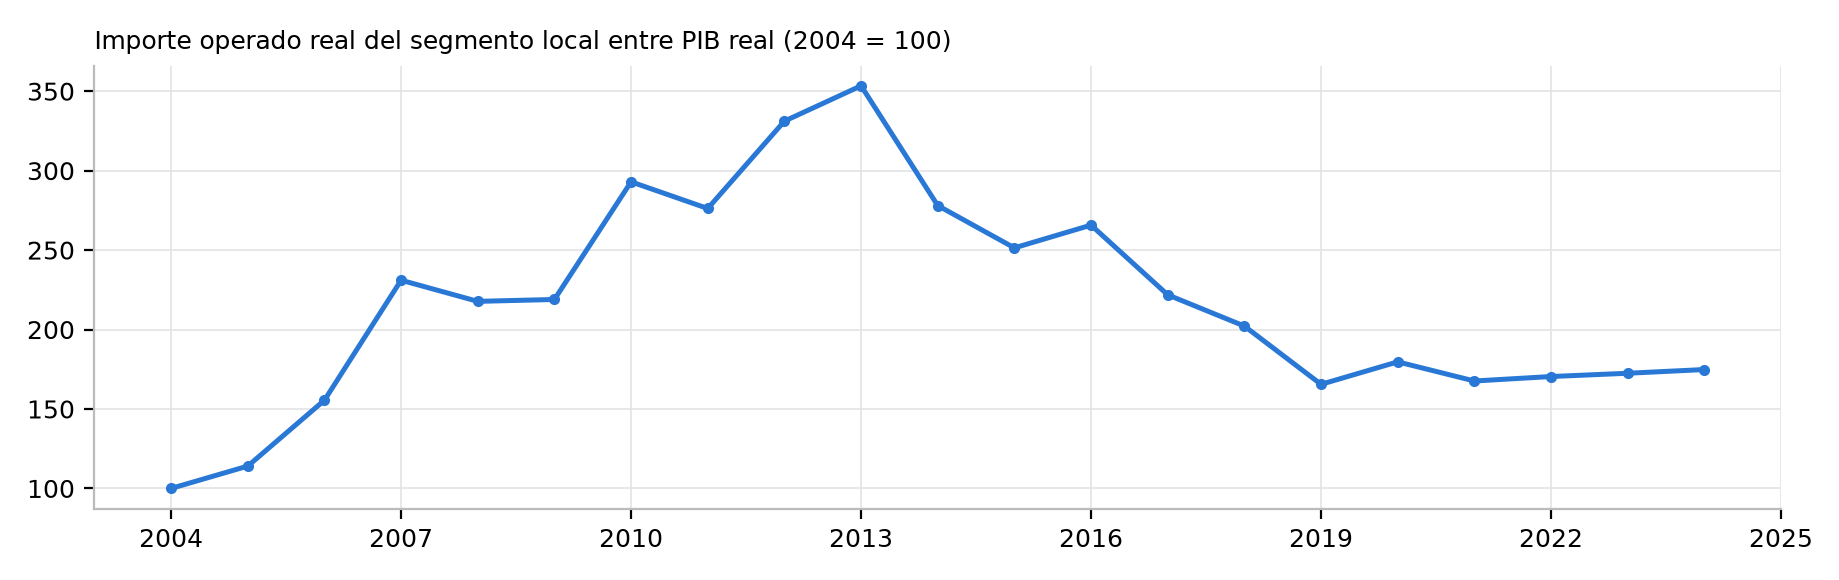
\includegraphics[width=\linewidth]{figuras/f2_local_pib.png}\end{center}

La razón se multiplica por \RrazonMultiplo\ entre 2004 y 2013 (índice \RratioDosMilTrece) y después pierde la mitad (\RratioDosMilVeinticuatro\ en 2024). El máximo de 2013 precede a enero de 2014, cuando entran juntos el impuesto de 10\% y la apertura del SIC al público (Sección~1). La historia del segmento local es una expansión de nueve años y una contracción de once.

\begin{cambio}
H1 se reformula como dos afirmaciones verificables: (i) la participación del SIC aumentó; (ii) la razón importe local/PIB disminuyó desde su máximo. Con los datos de la autora, (ii) se cumple desde 2013. La conclusión de la tesis de que la tercera condición de H1 ``no se cumple'' depende de comparar contra 2004. Las tasas deben reportarse con pendiente y con dos años de inicio.
\end{cambio}

\begin{ejercicios}
\item Demuestre que si $V_t=V_0e^{\beta t}$ exactamente, ambas tasas coinciden. Construya un ejemplo de diez años en que difieran en más de cinco puntos.
\item Calcule la elasticidad de $g^{\mathrm{ext}}_{a,b}$ respecto de $V_a$. ¿Por qué el problema es mayor cuando $b-a$ es pequeño?
\item Con la tabla, explique por qué en el SIC la tasa entre extremos de 2019--2025 es positiva y la pendiente negativa.
\end{ejercicios}

%======================================================================
\section{¿Tiene tendencia la participación?}

\subsection{El problema}
La tesis regresa $\PSIC_t$ mensual sobre el tiempo con errores HAC (cinco rezagos) y obtiene $t=\RtHAC$, es decir, \RpendHAC\ puntos por año. En la misma página, la prueba ADF no rechaza raíz unitaria y la KPSS rechaza estacionariedad.

\begin{proposicion}[Regresión espuria contra el tiempo]
Si $y_t=\alpha+\beta t+u_t$ con $u_t$ integrada de orden uno y $\beta=0$, el estadístico $t$ de $\hat\beta$ por mínimos cuadrados, con errores convencionales o con errores HAC de un número fijo de rezagos, no converge a una normal: diverge a tasa $\sqrt{T}$ (Durlauf y Phillips, 1988). La probabilidad de ``encontrar'' una tendencia significativa tiende a uno.
\end{proposicion}

La simulación lo hace concreto: para 2,000 caminatas aleatorias del mismo largo que la serie (273 meses), la regresión con errores HAC de cinco rezagos rechaza ``no hay tendencia'' al 5\% en el \RrwRechazo\% de los casos, con una mediana de $|t|=\RrwMediana$.

\begin{center}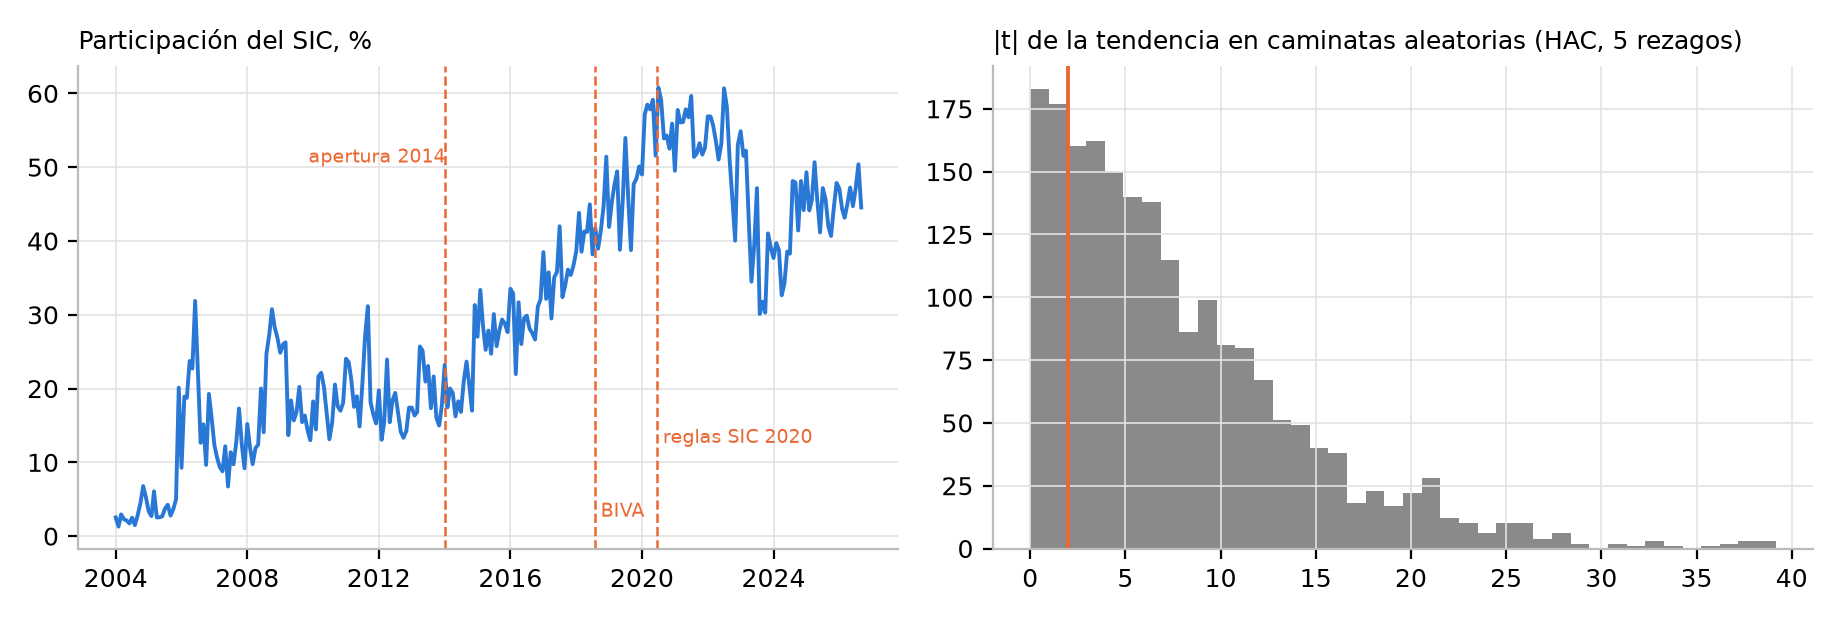
\includegraphics[width=\linewidth]{figuras/f1_tendencia.png}\end{center}

\subsection{Un contraste válido}
La participación está acotada en $(0,1)$, así que se trabaja con $\ell_t=\logit(\PSIC_t)=\ln\bigl(\PSIC_t/(1-\PSIC_t)\bigr)$. Para $\ell_t$, ADF da $p=\RadfLogit$ y KPSS con tendencia da $p=\RkpssLogit$: tampoco es estacionaria alrededor de una tendencia.

Si $\ell_t$ es una caminata aleatoria con deriva, $\Delta\ell_t=\mu+\varepsilon_t$, y ``hay tendencia'' significa $\mu>0$. El estimador $\bar{\Delta\ell}$ con error estándar de Newey--West (\RlagNW\ rezagos) es válido bajo raíz unitaria.

\begin{center}\small
\begin{tabular}{@{}lrr@{}}\toprule
Periodo & Deriva anual de $\logit(\PSIC)$ & $p$\\\midrule
2004--2026 & \RderivaAnual & \RpDeriva\\
2004--2013 & \RderivaA & \RpDerivaA\\
2014--2018 & \RderivaB & \RpDerivaB\\
2019--2026 & \RderivaC & \RpDerivaC\\\bottomrule
\end{tabular}
\end{center}

La deriva es positiva y económicamente grande (acumulada en 22 años lleva la participación de 3\% a 46\%), pero la serie es tan ruidosa que una sola trayectoria no permite distinguirla de cero. No es una contradicción. Que la participación subió es un hecho; que haya una tendencia estadística que la empuja es una inferencia, y con una sola historia de 22 años la inferencia es débil. El tramo con la deriva más clara es 2014--2018, justo después de la apertura de enero de 2014.

Alternativas formales que no exigen decidir antes si la serie es $I(0)$ o $I(1)$: Vogelsang (1998), Harvey, Leybourne y Taylor (2007) y Perron y Yabu (2009). Para quiebres en la tendencia, Kejriwal y Perron (2010). Las pruebas de Chow y el procedimiento de Bai y Perron (1998) suponen errores estacionarios y no deben aplicarse a $\PSIC_t$ en niveles. Además, las fechas de la Tabla 4.12 de la tesis no se reproducen con el algoritmo del cuaderno de la propia autora (cambio de nivel, mínimo de doce meses, criterio bayesiano): para la participación coinciden tres de cuatro fechas y para los indicadores de liquidez salen fechas distintas. Es un síntoma más de que esas fechas no deben sostener conclusiones.

\begin{cambio}
La afirmación ``la tendencia es significativa por dos vías'' se retira. Se reporta el aumento como hecho descriptivo, la deriva en diferencias con su intervalo, y las fechas de quiebre solo con un procedimiento robusto a raíz unitaria.
\end{cambio}

\begin{ejercicios}
\item Reproduzca la simulación con 1, 5 y 20 rezagos de Newey--West. ¿Mejora el tamaño de la prueba al aumentar los rezagos?
\item Demuestre que bajo $\Delta\ell_t=\mu+\varepsilon_t$ con $\varepsilon_t$ ruido blanco, $\operatorname{Var}(\bar{\Delta\ell})=\sigma^2/T$ y que $\ell_T-\ell_0=T\bar{\Delta\ell}$. ¿Qué implica sobre la información de una sola trayectoria?
\end{ejercicios}

%======================================================================
\section{Medidas de liquidez}

\subsection{Definiciones}
Para la serie $i$ en la sesión $d$ con rendimiento $R_{i,d}$, importe $V_{i,d}$ y posturas $A_{i,d},B_{i,d}$ al final de la sesión:
\begin{align*}
\SPREAD_{i,d}&=\frac{A_{i,d}-B_{i,d}}{(A_{i,d}+B_{i,d})/2},\qquad
\ILLIQ_{i,t}=\frac{1}{D_{i,t}}\sum_{d\in\mathcal D_{i,t}}\frac{|R_{i,d}|}{V_{i,d}},\\
\ZRET_{i,t}&=\frac{\#\{d:\text{sin operación}\}+\#\{d:\text{operada},\,R_{i,d}=0\}}{N^{\mathrm{vig}}_{i,t}-\#\{d:\text{operada, sin }R\}},\qquad
\TURN_{j,t}=\frac{\sum_{i\in j}V_{i,t}}{\overline{MC}_{j,t}}.
\end{align*}
El diferencial y Amihud miden costo; $\ZRET$ mezcla costo y ausencia de negociación; la rotación mide actividad, no costo (Lo y Wang, 2000).

\subsection{Unidades: Amihud debe deflactarse}
Si $V$ está en pesos corrientes, $\ILLIQ^{\mathrm{real}}_{t}=\ILLIQ^{\mathrm{nom}}_{t}\cdot P_t/P_{2018}$, con $P$ el INPC. En logaritmos, $\ln\ILLIQ^{\mathrm{real}}=\ln\ILLIQ^{\mathrm{nom}}+\ln(P_t/P_{2018})$. Con la mediana anual, entre 2004 y 2014 la mejora nominal es de $\RillNomA$ puntos logarítmicos y la real de $\RillRealA$; entre 2014 y 2025 el deterioro nominal es de $\RillNomB$ y el real de $\RillRealB$. La inflación exagera la mejora inicial y \emph{oculta} parte del deterioro reciente.

Hay dos maneras de quitar la escala monetaria: deflactar, o dividir cada año entre el promedio del mercado, como sugiere Amihud (2002). La segunda elimina además cualquier cambio común de nivel, así que sirve para comparar emisoras entre sí pero no para medir si el mercado en conjunto se volvió más o menos líquido. Kyle y Obizhaeva (2016) señalan otro problema de escala: $\ILLIQ$ depende del horizonte de medición, porque volumen y volatilidad escalan distinto con el tiempo. Al comparar la versión mensual con la anual, hay que tenerlo presente.

\subsection{Rendimientos cero: bimodalidad}
\begin{center}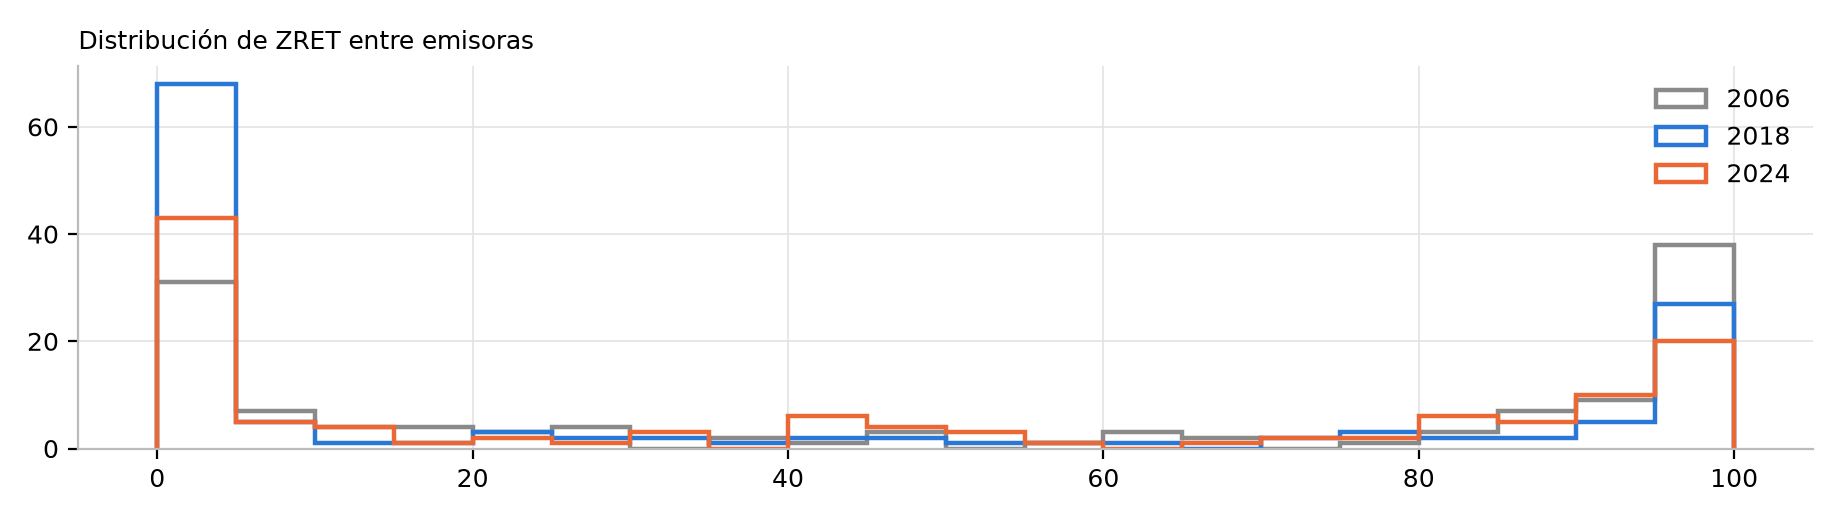
\includegraphics[width=\linewidth]{figuras/f4_zret_bimodal.png}\end{center}
La distribución de $\ZRET$ entre emisoras tiene dos masas: las que operan todos los días ($\ZRET\approx 0$) y las que casi no operan ($\ZRET$ cerca de 1). La mediana cae entre ambas y salta cuando unas cuantas empresas cambian de grupo. La mediana va de \RzMedA\% (2004) a \RzMedB\% (2018) y \RzMedC\% (2026); la media, de \RzMeanA\% a \RzMeanB\% y \RzMeanC\%. La forma de U existe, pero es mucho más tenue de lo que sugiere la mediana.

\begin{center}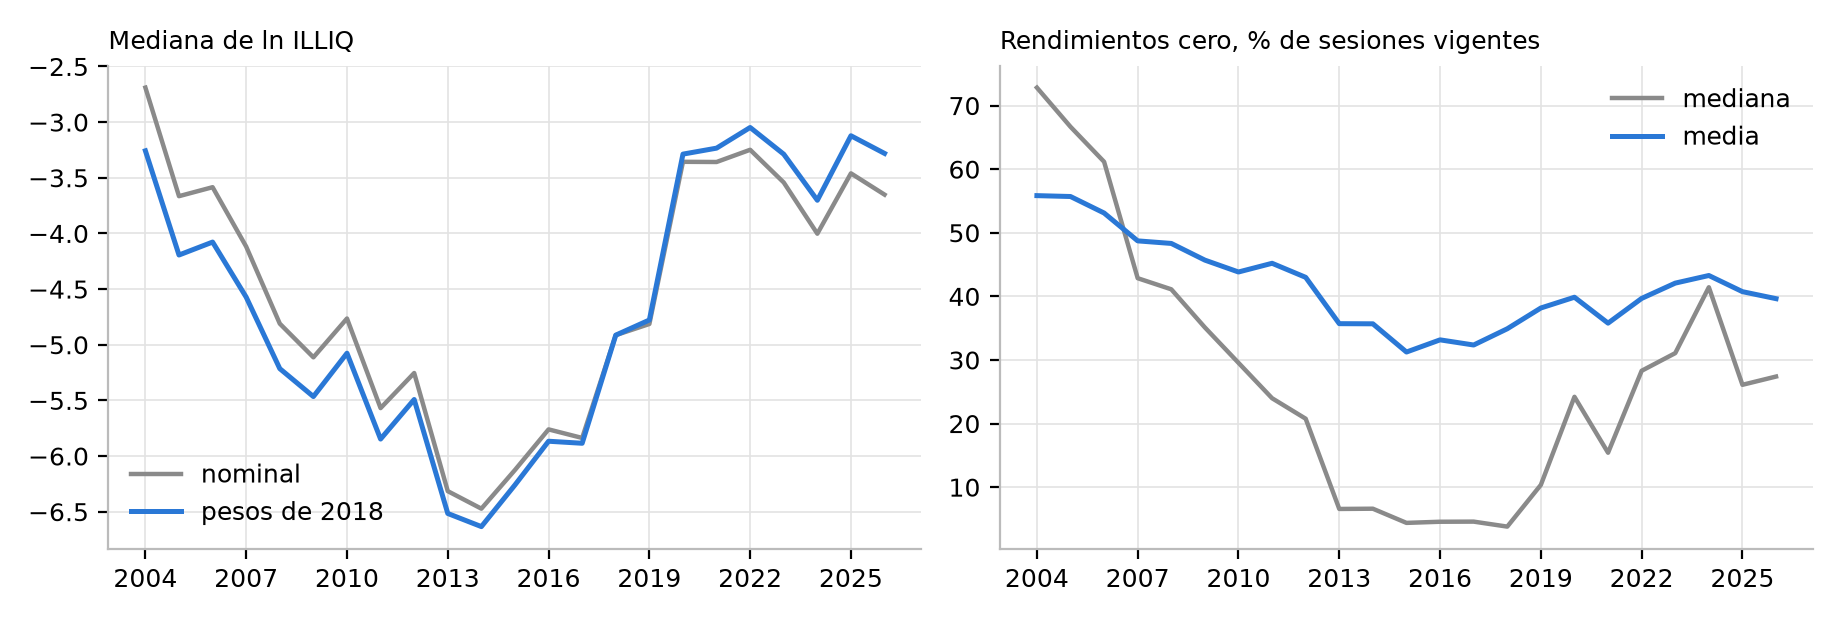
\includegraphics[width=\linewidth]{figuras/f3_medidas.png}\end{center}

\subsection{El proveedor también cambia}
Desde 2019 Bloomberg rellena el índice de rendimiento total en las sesiones sin operación con el último valor. La tesis lo detectó y por eso define la sesión sin operación por el importe, no por el precio: es la mejor decisión de medición del trabajo. Hay un segundo efecto que la tesis no reporta. Antes de 2019, la primera sesión operada después de una sin operación no tiene rendimiento medible y sale del denominador de $\ZRET$ (entre \RsinMedirMin\% y \RsinMedirMax\% de las sesiones operadas en 2014--2018); desde 2020 sale a lo sumo el \RsinMedirPost\%. Con una definición consistente (cada sesión operada contra la última sesión operada), la correlación con la medida de la tesis por empresa-año es \RcorrZalt. El aumento de $\ZRET$ después de 2018 es real, no un artefacto de esa regla.

Lo que sí cambia después de 2018 es la proporción de sesiones \emph{operadas} con rendimiento cero: \RceroOpA\% en 2018, \RceroOpB\% en 2019 y \RceroOpC\% en promedio en 2022--2025. Los cambios de 2020 a los cruces por excepción \emph{no} sirven de explicación: esas operaciones solo existen para valores del SIC (Sección~1.2). Una hipótesis que sí puede contrastarse es la llegada masiva de órdenes pequeñas de personas físicas en 2020--2021, que eleva la frecuencia de operaciones al mismo precio en emisoras poco negociadas. Hay evidencia para Estados Unidos de que el comportamiento gregario de inversionistas minoristas inexpertos reduce la liquidez por el riesgo de inventario que impone a quienes la proveen (Eaton, Green, Roseman y Wu, 2022). Para probarla se necesitan los boletines mensuales de la CNBV sobre casas de bolsa o datos por operación.

\subsection{El diferencial al final de la sesión y los estimadores de rango}
En la BMV el precio de cierre no sale de una subasta: es un promedio ponderado por volumen de las operaciones cercanas al final de la sesión, y existe un periodo de registro de posturas al precio de cierre\web{14}. Las posturas que reporta Bloomberg al final del día pueden por tanto no representar el costo de operar durante la sesión. Los estimadores de Corwin y Schultz (2012) y Abdi y Ranaldo (2017) correlacionan negativamente con ese diferencial en esta muestra. La tesis concluye que los estimadores fallan; lo correcto es que \emph{alguna} de las dos medidas falla y que, sin datos intradía, no se sabe cuál. La literatura de validación (Goyenko, Holden y Trzcinka, 2009; Fong, Holden y Trzcinka, 2017) compara contra un referente de alta frecuencia.

\begin{ejercicios}
\item Demuestre que la deflactación de $\ILLIQ$ no altera ninguna comparación entre emisoras dentro del mismo año, pero sí cualquier comparación entre años. ¿Qué pasa con la normalización por el promedio del mercado?
\item Con dos grupos de emisoras ($\ZRET=0.02$ y $\ZRET=0.9$) en proporciones $\pi$ y $1-\pi$, calcule la mediana y la media en función de $\pi$. ¿Para qué valores de $\pi$ es la mediana discontinua?
\end{ejercicios}

%======================================================================
\section{Comparar periodos y tamaños}

\subsection{La agregación por tramo puede borrar el cambio}
La tesis resume cada empresa con la mediana de sus valores anuales en cada tramo (2004--2013, 2014--2018, 2019--2025) y compara con Wilcoxon pareado. Para $\ZRET$, la mediana del cambio entre los dos primeros tramos es cero, mientras la mediana anual cae de \RzMedA\% (2004) a \RzMedTrece\% (2013). No es composición: entre las \RnPermanecen\ empresas presentes en 2004 y en 2018, la mediana cae de \RzPermA\ a \RzPermB. La caída ocurre \emph{dentro} del primer tramo, y la mediana de diez años la promedia. Regla práctica: un tramo largo solo es una unidad de comparación si la serie es aproximadamente plana dentro de él.

\subsection{La prueba de tamaño en la ventana correcta}
H2 dice que el deterioro afectó más a las emisoras pequeñas. El deterioro ocurre entre 2014--2018 y 2019--2025; la tesis prueba el tamaño entre 2004--2013 y 2019--2025. En esa ventana la única diferencia significativa es la rotación del tercil menor ($p$ ajustada por Holm \RrotTunoTres). En la ventana correcta:

\begin{table}[h]\centering\small
\caption{Cambio entre 2014--2018 y 2019--2025 por tercil (mediana del cambio por empresa). Puntos porcentuales, salvo $\ln\ILLIQ$ real. Mann--Whitney bilateral contra el tercil mayor; Holm sobre ocho pruebas.}
\begin{tabular}{@{}llcrrr@{}}\toprule
Indicador & Grupo & $n$ (grupo / mayor) & Cambio grupo & Cambio mayor & $p$ Holm\\\midrule
\tablainput{tabla_tamano}
\bottomrule\end{tabular}
\end{table}

Los signos van en la dirección de la hipótesis (las pequeñas empeoran más en Amihud, rendimientos cero y rotación), pero con 25 a 43 empresas por grupo no hay potencia para distinguirlo. La conclusión honesta es ``no se puede saber con estos datos'', no ``la hipótesis no se cumple''. Un diseño con más potencia usa todos los años y todas las empresas:
\[
L_{i,t}=\alpha_i+\lambda_t+\sum_{g\in\{\text{menor},\text{intermedia}\}}\beta_g\,\mathbf 1\{G_i=g\}\cdot\mathbf 1\{t\ge 2019\}+\varepsilon_{i,t},
\]
con errores agrupados por empresa y por mes (Cameron, Gelbach y Miller, 2011; Thompson, 2011).

\begin{cambio}
La Tabla 4.10 se sustituye por la de la ventana del deterioro, con $n$ por grupo y una frase sobre potencia. La Tabla 4.7 se acompaña de la media de $\ZRET$.
\end{cambio}

%======================================================================
\section{Una variable agregada en un panel}

\subsection{Cuánta información hay realmente}
$\PSIC_t$ toma el mismo valor para todas las emisoras en cada mes. En $L_{i,t}=\alpha_i+\beta\PSIC_t+\dots$, el coeficiente $\beta$ se identifica solo con la variación temporal: hay $T=273$ observaciones informativas, no las más de veinte mil filas del panel. Moulton (1990) cuantifica el exceso de confianza de los errores convencionales: con $\bar n$ empresas por mes, correlación intramensual de los residuos $\rho_u$ y de la variable $\rho_x=1$,
\[
\frac{\operatorname{Var}_{\mathrm{verdadera}}(\hat\beta)}{\operatorname{Var}_{\mathrm{MCO}}(\hat\beta)}\approx 1+(\bar n-1)\rho_u .
\]
Driscoll y Kraay (1998) corrige eso, pero no crea información que no hay.

\subsection{Por qué el $R^2$ intragrupo en niveles engaña}
La tesis compara cuánto sube el $R^2$ intragrupo al añadir la participación con cuánto sube al añadir seis controles, \emph{en niveles}. Hay tres defectos:
\begin{enumerate}[label=(\roman*)]
\item Las series son persistentes o integradas; en niveles el $R^2$ mide tendencias compartidas. Con las medianas mensuales y los mismos seis regresores comunes, el $R^2$ en niveles es \RlvRA\%, \RlvRB\%, \RlvRC\% y \RlvRD\% para diferencial, Amihud, rendimientos cero y rotación; en primeras diferencias es mucho menor (tabla siguiente).
\item Uno de los controles, la volatilidad idiosincrática, varía entre empresas dentro de cada mes y se construye con los mismos rendimientos que Amihud y $\ZRET$; explica variación que $\PSIC_t$ no puede tocar por construcción.
\item El incremento de $R^2$ depende del orden de entrada, y seis variables contra una no es una comparación entre factores.
\end{enumerate}

\subsection{La comparación correcta}
Si $\PSIC_t$ solo varía en el tiempo, la pregunta ``¿cuánto contribuye frente a los demás factores comunes?'' es una pregunta de series de tiempo. Se resume cada mes con la mediana transversal de cada indicador (meses con al menos \RnMin\ emisoras), se diferencian todas las series y se descompone el $R^2$ con el valor de Shapley--Owen (Huettner y Sunder, 2012):
\[
\phi_k=\sum_{S\subseteq K\setminus\{k\}}\frac{|S|!\,(m-|S|-1)!}{m!}\bigl[R^2(S\cup\{k\})-R^2(S)\bigr],\qquad \sum_k\phi_k=R^2(K).
\]
$\phi_k$ no depende de un orden de entrada y compara variable contra variable. Los intervalos se obtienen con remuestreo por bloques de doce meses.

\begin{table}[h]\centering\small
\caption{Contribución de la participación del SIC en primeras diferencias, \RmesIni\ a \RmesFin\ (\RnMeses\ meses). Regresores: $\Delta\PSIC$ (en múltiplos de 10 pp), rendimiento y volatilidad del IPC, VIX, Cetes 28 y logaritmo del tipo de cambio. $\phi_{\PSIC}$ y su intervalo en \% de la varianza; ``Diferencia'': $\phi_{\PSIC}$ menos el mayor $\phi$ de los controles, intervalo al 95\%. Coeficiente de $\Delta\PSIC$ con errores de Newey--West.}
\begin{tabular}{@{}lrrcccrr@{}}\toprule
Indicador & $R^2$ & $\phi_{\PSIC}$ & IC 95\% & Lugar & Diferencia & $\hat\beta_{\PSIC}$ & $p$\\\midrule
\tablainput{tabla_h3}
\bottomrule\end{tabular}
\end{table}

\begin{center}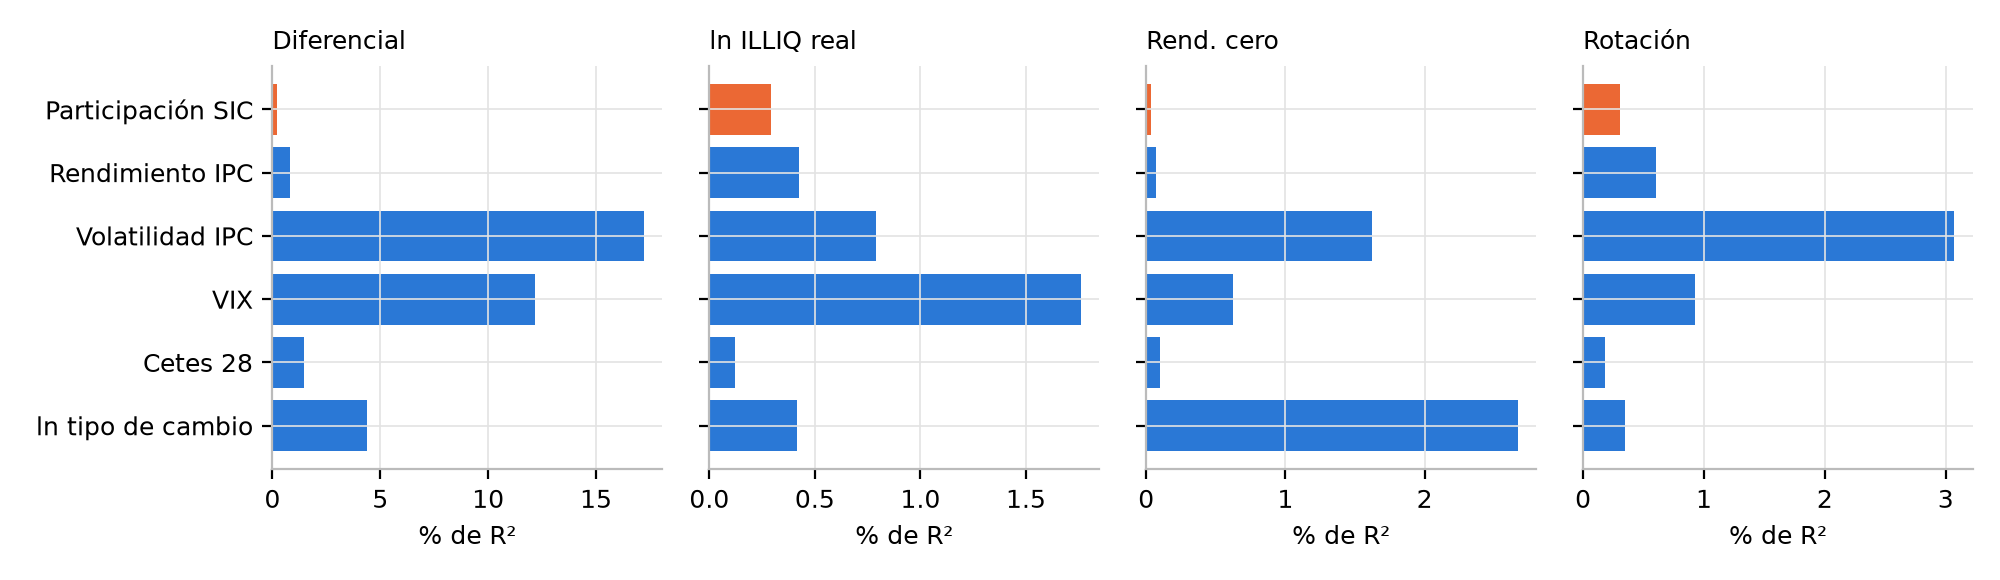
\includegraphics[width=\linewidth]{figuras/f5_shapley.png}\end{center}

Lectura: en los cuatro indicadores la participación aporta menos de un tercio de punto porcentual de la varianza mensual y ocupa el último o el penúltimo lugar entre seis factores. Su coeficiente no es significativo en ninguno. Para el diferencial y los rendimientos cero, el intervalo de la diferencia contra el control más importante excluye el cero: ahí la afirmación ``la participación contribuye menos que los factores financieros'' está respaldada. Para Amihud y rotación el intervalo incluye el cero: los controles también explican poco y los datos no ordenan a los factores.

\begin{cambio}
H3 se reformula con una regla de rechazo explícita: ``la contribución de Shapley de $\Delta\PSIC$ es menor que la del control común más importante''. Con esa regla se sostiene para el diferencial y los rendimientos cero y queda indeterminada para Amihud y rotación. Se retiran la comparación en niveles de la Tabla 4.13 y la razón ``480 a 1''. El coeficiente significativo de Amihud en el panel en diferencias de la tesis ($p=0.009$) se reproduce con el panel de la autora, pero no con medianas agregadas; la discrepancia debe discutirse, porque el panel pondera a cada empresa y la mediana no (Sección~7.4).
\end{cambio}

\subsection{El panel de la tesis, reestimado}
La autora descargó después el panel mensual de H3 (\texttt{m7\_panel\_mensual.parquet}). Con él, \texttt{scripts/verifica\_h3.py} reproduce las Tablas 4.11 y 4.15 a 4.17 hasta el redondeo, lo que habla bien del procedimiento, y resuelve las dos discrepancias abiertas: la razón del diferencial es 481 (la tabla dice 480; el texto, 473) y el valor $p$ de su coeficiente es 0.385 (la Tabla 4.11 dice 0.349; las demás, 0.387).

\begin{table}[h]\centering\small
\caption{Panel de la tesis reestimado: efectos fijos por emisora, tendencia, seis controles, errores de Driscoll--Kraay. Incrementos del $R^2$ intragrupo en puntos porcentuales sobre la misma muestra, en los dos órdenes de entrada.}
\begin{tabular}{@{}lrrrrrrr@{}}\toprule
& & & \multicolumn{3}{c}{Controles primero} & \multicolumn{2}{c}{Participación primero}\\
\cmidrule(lr){4-6}\cmidrule(l){7-8}
Indicador & $\hat\beta_{\PSIC}$ & $p$ & $\Delta R^2_{\mathrm{ctrl}}$ & $\Delta R^2_{\PSIC}$ & Razón & $\Delta R^2_{\PSIC}$ & Razón\\\midrule
\tablainput{tabla_panel}
\bottomrule\end{tabular}
\end{table}

La última columna muestra lo que la tesis no reporta: la razón depende del orden de entrada. Para Amihud baja de 15 a menos de 4 cuando la participación entra primero, porque ambos bloques comparten la tendencia. Es otra razón para usar la descomposición de Shapley--Owen, que promedia todos los órdenes.

La tesis promete estimar el modelo dentro de cada tercil y no lo reporta. Hecho con el mismo panel:

\begin{table}[h]\centering\small
\caption{Coeficiente de la participación por tercil de tamaño ($p$ de Driscoll--Kraay entre paréntesis).}
\begin{tabular}{@{}lcccc@{}}\toprule
Tercil & Diferencial & ln ILLIQ & Rend. cero & Rotación\\\midrule
\tablainput{tabla_tercil}
\bottomrule\end{tabular}
\end{table}

La asociación con los rendimientos cero vive casi entera en el tercil menor; la de rotación, en el mayor. Es el único indicio, en toda la evidencia de la tesis, de que la relación con el SIC difiere por tamaño, y conecta H2 con H3. Como todo coeficiente en niveles de este panel, es co-movimiento y no efecto: su versión en primeras diferencias por tercil es el siguiente paso.

\begin{ejercicios}
\item Demuestre que $\sum_k\phi_k=R^2(K)$ y que, si los regresores son ortogonales, $\phi_k$ es el $R^2$ de la regresión simple sobre $x_k$.
\item Explique por qué incluir efectos fijos de mes vuelve inidentificable a $\beta$ en $L_{i,t}=\alpha_i+\lambda_t+\beta\PSIC_t+\varepsilon_{i,t}$.
\item ¿Qué supuesto adicional necesitaría la regresión agregada para interpretar $\hat\beta_{\PSIC}$ como efecto causal? Dé un factor omitido plausible con la cronología de la Sección~1.
\end{ejercicios}

%======================================================================
\section{Identificación: lo que sí se puede hacer}
Con un único regresor agregado no hay manera de separar el efecto del SIC de cualquier otro choque común. Se necesita variación \emph{entre empresas} en la exposición al SIC, o un cambio institucional que afecte a unos y no a otros. Cuatro diseños factibles:
\begin{enumerate}
\item \textbf{Sustitución por índice.} Las emisoras del IPC compiten con el NAFTRAC y con ETF del SIC que replican mercados amplios; las que no están en el índice compiten menos. Estimar $L_{i,t}=\alpha_i+\lambda_t+\gamma\,\mathbf 1\{i\in\mathrm{IPC}\}\cdot\PSIC_t+\varepsilon_{i,t}$: los efectos de mes absorben todo lo común y $\gamma$ se identifica con la diferencia entre grupos.
\item \textbf{Sustitución sectorial.} Exposición de cada emisora al importe del SIC en su mismo sector GICS.
\item \textbf{La apertura de enero de 2014.} El público minorista gana acceso al SIC, pero el impuesto de 10\% se aplica a la vez a acciones locales y del SIC, así que su efecto relativo se cancela entre segmentos. Comparar emisoras con alta y baja participación previa de personas físicas aísla mejor el canal de sustitución.
\item \textbf{Eventos de listado.} Fechas de listado en el SIC de ETF amplios; comparar la liquidez de emisoras más y menos sustituibles alrededor de esas fechas.
\end{enumerate}
La cronología relevante no es la política sino la de microestructura y regulación (Sección~1). Las elecciones, la influenza o el aeropuerto de Texcoco de la Tabla 2.4 de la tesis no actúan sobre el mercado por un canal identificable.

%======================================================================
\section{Reproducibilidad}
\begin{itemize}
\item \textbf{Un solo procedimiento.} El cuaderno descargado (\texttt{Tesis\_procedimiento\_de\_calculo.ipynb}) es una versión anterior y no reproduce la tesis. El procedimiento que sí la reproduce está reconstruido y validado en \texttt{pipeline/}, módulo por módulo.
\item \textbf{Archivos identificados.} Hay cinco versiones del universo en Excel (1.4 GB) y siete duplicados exactos. La tabla \texttt{pipeline/archivos\_entrada.csv} da nombre, fecha, SHA-256 y papel de cada archivo; solo tres libros de Bloomberg y el libro de índices entran en los cálculos.
\item \textbf{Cifras generadas.} Este documento lee sus cifras de \texttt{resultados.tex} y de las tablas que genera \texttt{scripts/notas\_analisis.py}. Si los datos cambian, se vuelve a correr el script y el texto se actualiza solo. La tesis puede hacer lo mismo y eliminar de raíz las discrepancias entre texto y tablas: las dos que había (473 contra 480, 0.349 contra 0.387) eran errores de transcripción, no de cálculo (Sección~7.4).
\item \textbf{Datos con licencia.} Las extracciones de Bloomberg no se suben al repositorio; sí el código y los agregados que no reproducen precios.
\end{itemize}

%======================================================================
\section{Qué se necesita para cerrar}
\begin{enumerate}
\item \textbf{De la autora.} Nada indispensable. El procedimiento completo, de los libros de Bloomberg al panel de H3, ya está reconstruido en \texttt{pipeline/} y reproduce sus salidas (\texttt{pipeline/README.md}); la tabla de archivos de entrada con huella SHA-256 está en \texttt{pipeline/archivos\_entrada.csv}. La única entrada que no sale de los libros descargados es el mapa serie--empresa (identificador ID\_BB\_COMPANY de la terminal), que la autora ya generó. Su código original sigue siendo deseable para documentar la tesis.
\item \textbf{Decisiones de dirección.} Adoptar las reformulaciones de H1 (razón al PIB), H2 (ventana del deterioro, potencia declarada) y H3 (Shapley en diferencias con regla de rechazo). Decidir si la tesis incorpora uno de los diseños de identificación de la Sección~8 o lo deja como trabajo futuro.
\item \textbf{Documentos primarios.} Ya consultados: la LMV consolidada (derogación del artículo 264), las Reglas Operativas v1.53, v1.61, v1.69, v1.74 y v1.78, y el texto del DOF del 25 de octubre de 2024. Pendientes: el texto derogado del artículo 264 (está en la continuación del decreto del 10 de enero de 2014, en otra sección del DOF) y las versiones v1.70 a v1.73 para fechar el cambio de los cruces al día. Al citarse en la tesis, las fuentes periodísticas de la Sección~1 deben sustituirse por los documentos primarios.
\item \textbf{Datos nuevos.} Los boletines mensuales de la CNBV sobre casas de bolsa (número de contratos), para contrastar la hipótesis minorista. Los importes del SIC separados en acciones, ETF de renta variable y ETF de deuda (las extracciones de Bloomberg ya traen el tipo de valor). Si es posible, datos intradía de la BMV para validar el diferencial al final de la sesión.
\end{enumerate}

%======================================================================
\section{Resumen: de la tesis a la versión corregida}
\begin{center}\small
\begin{longtable}{@{}p{0.43\linewidth}p{0.52\linewidth}@{}}\toprule
Afirmación de la tesis (6 nov.\ 2026) & Versión corregida\\\midrule\endhead
El SIC se incorporó en 2003. & Creado el 14 de abril de 1997, relanzado en mayo de 2003, abierto a cualquier inversionista en enero de 2014.\\
El quiebre de 2014 se debe a ``la reforma que modificó las condiciones de acceso''. & En enero de 2014 coinciden la apertura del SIC y el impuesto de 10\% (que alcanza a ambos segmentos); en noviembre, el anonimato. No se pueden separar.\\
Participación de 1.13\% en 2004 (AMIB). & La AMIB no duplica el SIC en 2004; con convención homogénea, \RamibCorregido\%.\\
El SIC supera a ``todas las emisoras mexicanas''. & Solo frente al segmento local por domicilio, que incluye ETF y FIBRAs.\\
El local creció por encima del PIB en 21 años. & Solo contra 2004. Con pendientes crece como el PIB; desde 2013 se contrae, y la razón al PIB cae a la mitad.\\
Tendencia significativa ($t=\RtHAC$). & Inválido con raíz unitaria (\RrwRechazo\% de rechazos en caminatas aleatorias). Deriva positiva, no significativa ($p=\RpDeriva$).\\
Sin explicación para el máximo de 2020--2021. & Coincide con la triplicación de cuentas de personas físicas y con la ampliación de los márgenes de operación del SIC en junio y diciembre de 2020.\\
(Primera versión de estas notas) Los cruces de 2020 explicarían los rendimientos cero locales. & Retirado: los cruces por excepción solo existen para valores del SIC.\\
(Primera versión de estas notas) Las Afores ampliaron en 2024 su límite en valores extranjeros. & Retirado: sigue en 20\%. Lo que cambió fue el de estructurados (hasta 30\%, diferido) y el de divisas (de 35\% a 15\% según el DOF).\\
Fechas de quiebre (Tabla 4.12). & No se reproducen con el algoritmo de la autora; no deben sostener conclusiones.\\
(Hallazgo de la reconstrucción) Volatilidad idiosincrática. & Desde 2019 incluye sesiones sin operación con índice arrastrado y queda entre 10\% y 13\% por debajo; los coeficientes de H3 casi no cambian (\texttt{pipeline/README.md}).\\
Amihud mejora y luego empeora. & Igual en pesos reales; la inflación exagera la mejora y oculta parte del deterioro.\\
$\ZRET$ cae de 72.8\% a 3.8\%. & La mediana exagera por bimodalidad; la media va de \RzMeanA\% a \RzMeanB\%. El aumento posterior a 2018 es real.\\
Una diferencia por tamaño significativa (rotación). & Era la ventana equivocada; en la del deterioro ninguna es significativa, por falta de potencia.\\
H3 respaldada en los cuatro indicadores (niveles). & En diferencias y con Shapley--Owen: respaldada para diferencial y rendimientos cero; indeterminada para Amihud y rotación.\\
Razón de 473 a 1; $p=0.349$ (Tabla 4.11). & Errores de transcripción: 481 y 0.385 al reestimar con el panel de la autora. La razón depende además del orden de entrada.\\
(No reportado) Modelo por tercil. & La asociación con los rendimientos cero se concentra en las emisoras pequeñas.\\
Diferencial ``al cierre'' como referencia. & El cierre de la BMV es un promedio ponderado, no una subasta; las posturas del final del día son una referencia débil.\\\bottomrule
\end{longtable}
\end{center}

\section*{Referencias académicas}
\addcontentsline{toc}{section}{Referencias}
\begin{itemize}[leftmargin=*,label={}]\raggedright\small
\item Abdi, F. y Ranaldo, A. (2017). A simple estimation of bid-ask spreads from daily close, high, and low prices. \emph{The Review of Financial Studies, 30}(12), 4437--4480.
\item Amihud, Y. (2002). Illiquidity and stock returns: Cross-section and time-series effects. \emph{Journal of Financial Markets, 5}(1), 31--56.
\item Bai, J. y Perron, P. (1998). Estimating and testing linear models with multiple structural changes. \emph{Econometrica, 66}(1), 47--78.
\item Cameron, A. C., Gelbach, J. B. y Miller, D. L. (2011). Robust inference with multiway clustering. \emph{Journal of Business \& Economic Statistics, 29}(2), 238--249.
\item Corwin, S. A. y Schultz, P. (2012). A simple way to estimate bid-ask spreads from daily high and low prices. \emph{The Journal of Finance, 67}(2), 719--760.
\item Driscoll, J. C. y Kraay, A. C. (1998). Consistent covariance matrix estimation with spatially dependent panel data. \emph{The Review of Economics and Statistics, 80}(4), 549--560.
\item Durlauf, S. N. y Phillips, P. C. B. (1988). Trends versus random walks in time series analysis. \emph{Econometrica, 56}(6), 1333--1354.
\item Eaton, G. W., Green, T. C., Roseman, B. S. y Wu, Y. (2022). Retail trader sophistication and stock market quality: Evidence from brokerage outages. \emph{Journal of Financial Economics, 146}(2), 502--528.
\item Fong, K. Y. L., Holden, C. W. y Trzcinka, C. A. (2017). What are the best liquidity proxies for global research? \emph{Review of Finance, 21}(4), 1355--1401.
\item Goyenko, R. Y., Holden, C. W. y Trzcinka, C. A. (2009). Do liquidity measures measure liquidity? \emph{Journal of Financial Economics, 92}(2), 153--181.
\item Harvey, D. I., Leybourne, S. J. y Taylor, A. M. R. (2007). A simple, robust and powerful test of the trend hypothesis. \emph{Journal of Econometrics, 141}(2), 1302--1330.
\item Huettner, F. y Sunder, M. (2012). Axiomatic arguments for decomposing goodness of fit according to Shapley and Owen values. \emph{Electronic Journal of Statistics, 6}, 1239--1250.
\item Kejriwal, M. y Perron, P. (2010). A sequential procedure to determine the number of breaks in trend with an integrated or stationary noise component. \emph{Journal of Time Series Analysis, 31}(5), 305--328.
\item Kyle, A. S. y Obizhaeva, A. A. (2016). Market microstructure invariance: Empirical hypotheses. \emph{Econometrica, 84}(4), 1345--1404.
\item Lo, A. W. y Wang, J. (2000). Trading volume: Definitions, data analysis, and implications of portfolio theory. \emph{The Review of Financial Studies, 13}(2), 257--300.
\item Moulton, B. R. (1990). An illustration of a pitfall in estimating the effects of aggregate variables on micro units. \emph{The Review of Economics and Statistics, 72}(2), 334--338.
\item Perron, P. y Yabu, T. (2009). Estimating deterministic trends with an integrated or stationary noise component. \emph{Journal of Econometrics, 151}(1), 56--69.
\item Thompson, S. B. (2011). Simple formulas for standard errors that cluster by both firm and time. \emph{Journal of Financial Economics, 99}(1), 1--10.
\item Vogelsang, T. J. (1998). Trend function hypothesis testing in the presence of serial correlation. \emph{Econometrica, 66}(1), 123--148.
\end{itemize}

\section*{Fuentes públicas consultadas (9 de noviembre de 2026)}
\begin{enumerate}[label={[\arabic*]},leftmargin=*]\raggedright\small
\item Bolsa Mexicana de Valores, documento corporativo sobre el SIC (inicio el 14 de abril de 1997; apertura a todo inversionista desde enero de 2014). \url{https://gruporeforma.reforma.com/Libre/Offlines/Mty/PerfilEmpresarial/img/Reportes/PDF/296.pdf}
\item Expansión (2023, 23 de septiembre). ¿Qué es el SIC en la Bolsa de Valores? \url{https://expansion.mx/mercados/2023/09/23/sistema-internacional-de-cotizaciones-bmv-20-anos}
\item El Financiero. ``Ventana'' global de la BMV cumple 15 años. \url{https://www.elfinanciero.com.mx/mercados/ventana-global-de-la-bmv-cumple-15-anos/}
\item Ley del Mercado de Valores, artículos 262 a 264. \url{https://www.diputados.gob.mx/LeyesBiblio/pdf/LMV.pdf}
\item SAT, criterio normativo 37/ISR/N, enajenación de acciones de sociedades extranjeras en bolsas concesionadas. \url{https://wwwmat.sat.gob.mx/articulo/50782/criterio-46/isr/n}
\item Artículo 129 de la Ley del ISR (compendio). \url{https://sdv.com.mx/compendio/ley-isr/articulo-129/}
\item CNBV (2021). Comunicado 59: información de las 35 casas de bolsa a marzo de 2021. \url{https://www.gob.mx/cnbv/prensa/comunicado-no-59-informacion-estadistica-y-financiera-de-las-35-casas-de-bolsa-a-marzo-de-2021-273669?idiom=es}
\item La Jornada (2021, 8 de septiembre). CNBV: crecen 33\% en un año inversionistas en Bolsa. \url{https://www.jornada.com.mx/2021/09/08/economia/024n1eco}
\item Grupo BMV, Informe Anual 2021 (ampliación de horarios de cruces por excepción en valores del SIC). \url{https://www.bmv.com.mx/docs-pub/sustenta/sustenta_1185846_2021_1.pdf}
\item Grupo BMV (2022, 4 de enero). 3 mil valores listados en el SIC. \url{https://www.bmv.com.mx/docs-pub/SALA_PRENSA/CTEN_BOLE/3\%20mil\%20valores\%20listados\%20en\%20el\%20SIC\%20de\%20BMV\%20040122.pdf}
\item Funds Society (2022). Participación del SIC en el importe de la BMV según la AMIB. \url{https://www.fundssociety.com/es/?p=115098}
\item El CEO. Consar: el régimen de inversión del Sistema de Ahorro para el Retiro. \url{https://elceo.com/opinion/consar-regimen-inversion-sistema-ahorro-para-el-retiro/}
\item El CEO. BMV registra el menor número de empresas listadas en casi 20 años. \url{https://elceo.com/mercados/bmv-registra-el-menor-numero-de-empresas-listadas-en-casi-20-anos/}
\item BMV, Reglamento Interior (definición del precio de cierre). \url{https://www.bmv.com.mx/docs-pub/MARCO_NORMATIVO/CTEN_MNRST/REGLAMENTO\%20INTERIOR\%20BMV\%20VIGENTE-10092018-Reg.\%20D.A..pdf}
\item Bolsa Mexicana de Valores (2017). Reglas Operativas del Sistema Electrónico de Negociación, versión 1.53, vigente desde el 22 de mayo de 2017. \url{https://www.bmv.com.mx/docs-pub/MARCO_NORMATIVO/CTEN_MERMO/20170522_V1%2053_Filtros%20valores%20menores%20a%20un%20peso_(Esp).pdf}
\item Bolsa Mexicana de Valores (2020). Reglas Operativas, versión 1.74, vigente desde el 15 de junio de 2020 (filtros en SIC al 8\%). \url{https://bmv.com.mx/docs-pub/MARCO_NORMATIVO/CTEN_MERMO/20200615_V1.74_Filtros%20en%20SIC%20al%208%20%20(ESP).pdf}
\item Bolsa Mexicana de Valores (2020). Reglas Operativas, versión 1.78, vigente desde el 16 de diciembre de 2020 (rangos estáticos en SIC). \url{https://www.bmv.com.mx/docs-pub/MARCO_NORMATIVO/CTEN_MERMO/20201216_V1.78_Rangos%20est%C3%A1ticos%20en%20SIC%20(ESP).pdf}
\item CONSAR. Límites del régimen de inversión (aplicables desde el 28 de octubre de 2024; consulta del 9 de noviembre de 2026). \url{https://www.consar.gob.mx/gobmx/aplicativo/limites_inversion/}
\item Moody's Local México (2024, 28 de octubre). Mejoras en el régimen de inversión de las Afores. \url{https://moodyslocal.com.mx/wp-content/uploads/2024/10/3.1_MLMX_Research_RegimendeInversion_28102024_VFF.pdf}
\item SHCP (2024, 25 de octubre). Modificaciones y adiciones a las Disposiciones de carácter general que establecen el régimen de inversión al que deberán sujetarse las Sociedades de Inversión Especializadas de Fondos para el Retiro. Diario Oficial de la Federación (texto en SIDOF). \url{https://sidof.segob.gob.mx/notas/docFuente/5741711}
\item Bolsa Mexicana de Valores (2018). Reglas Operativas, versión 1.61, vigente desde el 30 de julio de 2018. \url{https://www.bmv.com.mx/docs-pub/MARCO_NORMATIVO/CTEN_MERMO/20180730_V1%2061_Subastas%20VM%20(Esp).pdf}
\item Bolsa Mexicana de Valores (2019). Electronic Trading System Rules, versión 1.69, vigente desde el 1 de noviembre de 2019. \url{https://www.bmv.com.mx/docs-pub/MARCO_NORMATIVO/CTEN_MERMO/20191101_V1.69_RINO%202019.04_Nuevas%20Cuotas%20Operativas%20(ING).pdf}
\item Bolsa Mexicana de Valores (2020). Electronic Trading System Rules, versión 1.71, vigente desde el 6 de abril de 2020. \url{https://www.bmv.com.mx/docs-pub/MARCO_NORMATIVO/CTEN_MERMO/20200406_V1.71_Operaciones%20al%20INAV%20(ING).pdf}
\end{enumerate}
\small Las fuentes periodísticas sirven para fechar hechos; para citarlos en la tesis conviene ir al documento primario (DOF, informes anuales de la BMV, boletines de la CNBV).

\end{document}
